
\mySection{13.1 Introduction}
%-------------- start slide -------------------------------%{{{ 13.4
\begin{frame}
	% {\S\: 13.1 Introduction}
	\begin{center}
		{\bf Rationale:}\\[1em]Reducing variability by blocking$^\dagger$
		\vfill
		{\small {\it $^\dagger$ Blocking} is the arranging of experimental units in groups (blocks) that are similar to one another.}
		\vfill
		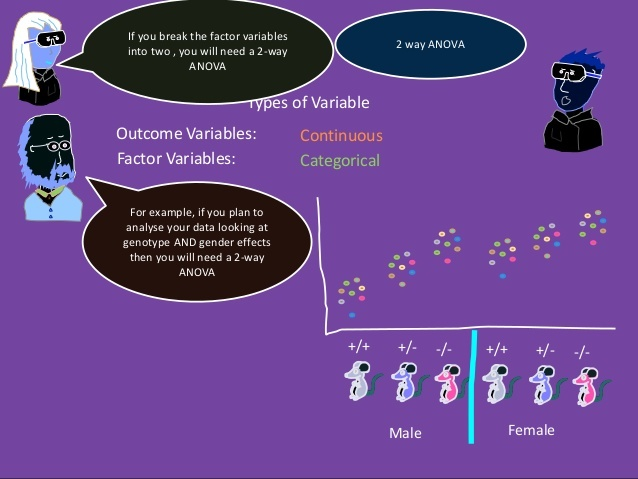
\includegraphics[scale=0.25]{experimental-design-cartoon-neg.jpg}
		\vfill
		{\footnotesize
		\url{https://www.slideshare.net/KevinHamill2/experimental-design-cartoon-part-5-sample-size}}
	\end{center}
\end{frame}
%-------------- end slide -------------------------------%}}}
%-------------- start slide -------------------------------%{{{ 13.5
\begin{frame}[fragile]
	\centering
	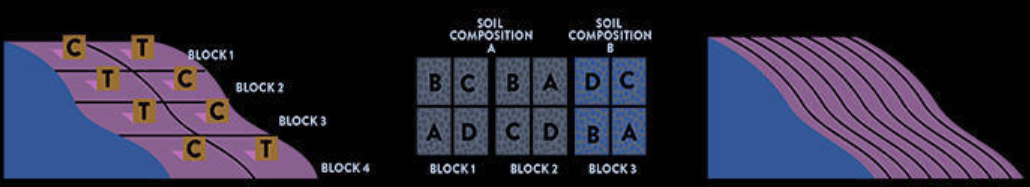
\includegraphics[scale=0.3]{Addressing-Field.png}
	\vfill

	\begin{minipage}{0.6\textwidth}
	\begin{enumerate}
	\item[Goal] Reducing variability caused by
	\item[a]  {\it elevation}.
	\item[b]  {\it soil types}.
	\item[]  \qquad {v.s.}
	\item[c] {\it complete randomized design}
	\end{enumerate}
	\end{minipage}
\hfill\pause
	\begin{minipage}{0.35\textwidth}
		\vspace{1.8em}
	\begin{enumerate}
	\item[]
		$\scalebox{2.2}{\}}$\hfill One-way ANOVA
		% \[
		% \scalebox{2.2}{\}}\:\text{One-way ANOVA}
		% \]
		\vspace{1.4em}
	\item[]\hfill Two-way ANOVA
	\end{enumerate}
	\end{minipage}

	\vfill
	{\footnotesize\url{https://www.sare.org/Learning-Center/Bulletins/How-to-Conduct-Research-on-Your-Farm-or-Ranch/Text-Version/Basics-of-Experimental-Design}}
\end{frame}
%-------------- end slide -------------------------------%}}}
